\documentclass[conference]{IEEEtran}
\makeatletter
\newcommand{\rmnum}[1]{\romannumeral #1}
\newcommand{\Rmnum}[1]{\expandafter\@slowromancap\romannumeral #1@}
\makeatother

\usepackage{epsfig}
\usepackage{amsopn}
\usepackage{subfigure}
\usepackage{cite}
\ifCLASSINFOpdf

\else
\fi
\usepackage[cmex10]{amsmath}

\interdisplaylinepenalty = 2500

\usepackage{algorithmic}
\usepackage{algorithm}
\hyphenation{op-tical net-works semi-conduc-tor}


\begin{document}
\title{Access Strategy in Super WiFi Network Powered by Solar Energy Harvesting, A POMDP Method}

\author{\authorblockN{Tingwu~Wang\authorrefmark{1},
	Chunxiao~Jiang\authorrefmark{1},
	Yan~Chen\authorrefmark{2},
	Yong~Ren\authorrefmark{1}, and
	K. J. Ray~Liu\authorrefmark{2}}
	\small\authorblockA{\authorrefmark{1}
		Department of Electronic Engineering, Tsinghua University, Beijing, 100084, P. R. China\\
          \authorrefmark{2}Department of Electrical and Computer Engineering,
		  University of Maryland, College Park, MD 20742, USA\\
        E-mail: wtw12@mails.tsinghua.edu.cn, \{jchx, reny\}@tsinghua.edu.cn, \{yan, kjrliu\}@umd.edu}}
\maketitle

\begin{abstract}
The recently announced Super Wi-Fi Network proposal is aiming to enable Internet access in a nation-wide area.
As traditional cable-connected power supply system becomes impractical or costly for a wide range wireless network,
new infrastructure deployment for Super Wi-Fi is needed.
The fast developing Energy Harvesting (EH) techniques receive global 
concerns for their potential of solving the above power supply problem. 
Many studies have been done on traditional access strategy,
but the access strategy in EH wireless network with multiple Base Stations (BS)
remains a field with no in-depth researches.
Different from traditional wireless network,
a Base Station (BS) in EH powered network harvests energy from the ambient environment.
And as the energy is limited, 
the BS will not broadcast its system state to all the users within its range,
which provides incomplete information for the users. 
Thus the access strategy has to be carefully chosen.
In this paper, we propose a practical and efficient framework for multiple BSs access strategy
in an EH powered Super Wi-Fi network.
In our work, we consider the access strategy from the opportunistic user (OU) perspective,
who exploits downlink transmission opportunities with the Passive Users (PU).
To formulate the problem,
we used Partially Observable Markov Decision Process (POMDP) to model the
real world uncertainty.
Simulation results show that our methods are efficacious and significantly outperforms
the traditional widely used CSMA method.
\end{abstract}
\IEEEpeerreviewmaketitle
\section{Introduction}
% ------------------------------------------------------------------------------------------- %
% background
In order to expand the coverage area of wireless network,
many algorithms and implementations have been revised.
And recently, the Federal Communications Commission published the Super Wi-Fi proposal,
aiming to make use of lower-frequency white spaces between television channel frequencies
and create a nationwide wireless network.
However, the ambitious task of building a countrywide network comes across many obstacles.
An inevitable problem is how to deploy practical backhaul and energy supply system.
Traditional cable-based systems are excessive, considering the cost for deploying and maintaining the network,
and sometimes impossible as well as dangerous in complex environment.
Despite all the above difficulties, there are solutions and
many successful experimental deployments of Super Wi-Fi are accomplished accordingly.
Wireless backhual has been proven to be effective \cite{30} as a replacement for cable backhaul.
And the fast developing EH technology provides an ideal replacement as the power supply problem, 
which could make use of a wide range of ambient energy including piezoelectric, thermal, solar energy, etc.\\
% ------------------------------------------------------------------------------------------- %
% previous work
\indent As the deployment of EH network is just emerging,
new wireless protocols and modification are needed, as some preliminary studies pointed out \cite{27}.
Previously, the access strategy problem has been a core problem in wireless communications,
and many researchers have been doing some brilliant work in the literature.
Markov Decision Process have been widely used in wireless network,
with some challenges and solutions summarized in \cite{23}.
Access process is a typical game process,
and therefore game theory, summarized in \cite{22},
and pricing theory, used in \cite{7}, has been applied respectively.
In \cite{5}, the access strategy towards multiple BSs with negative externality is considered.
More recently, a POMDP MAC layer opportunistic access is proposed by Dr. Zhao in \cite{zhao1}.
A learning based approach to access between packet bursts is studied in \cite{kae1}.
\\
% ------------------------------------------------------------------------------------------- %
% our work
\indent However, the mentioned existing studies on the access strategy considered infinite or always sufficient battery supply.
%
% ---------------------------------------------------- %
% 	first
First, most of them assume infinite or always sufficient battery supply.
As mentioned above, in building the wide range Super Wi-Fi network,
using BSs with limited battery and constantly energy exhaust is unavoidable.
% 	second
Second, in many of the works,
the number of users and the remaining battery is static or assumed to be changing slowly.
The corresponding algorithms would generate out-of-time strategy as the BS states are changing rapidly in real practice.
And learning based algorithms may merely be oscillating and converges to meaningless results.
% 	third
Third, the influence of the OUs on the BS, is neglected.
When a OU makes a decision, it inevitably affects system state.
For example, the OU could cause energy exhaust,
collision and system low efficiency if it performs short-sighted and selfish strategy,
or causing energy waste when it is too conservative.
%	fourth
Fourthly, the full knowledge of the system is unrealistic.
The assumption that the decision maker has the full knowledge will make the model simple,
but will make the implementation in real life irrealizable.
% conclusion about our model
In this work, we propose an algorithm that is able to overcome the aformentioned drawbacks.
And although our work focuses on solar energy harvesting,
it is clear that the conclusion and the algorithm could be generalize to any AP selection problem in EH powered network.
\\
% ------------------------------------------------------------------------------------------- %
% organization
\indent The rest of this paper is organized as follow.
We describe the system model In Section \Rmnum{2}.
And in Section \Rmnum{3}, the POMDP formulation is presented,
showing how we abstract the continuous battery state and user state to
POMDP states and draws the optimal decision. And a suboptimal strategy is proposed.
In Section \Rmnum{4}, we evaluate the performance of our proposed approach with several famous traditional algorithm.
Finally, Section \Rmnum{5} draws the conclusion.
% ------------------------------------------------------------------------------------------- %
% ----------------------------end of introduction-------------------------------------------- %
% ------------------------------------------------------------------------------------------- %
\begin{figure}
\centering
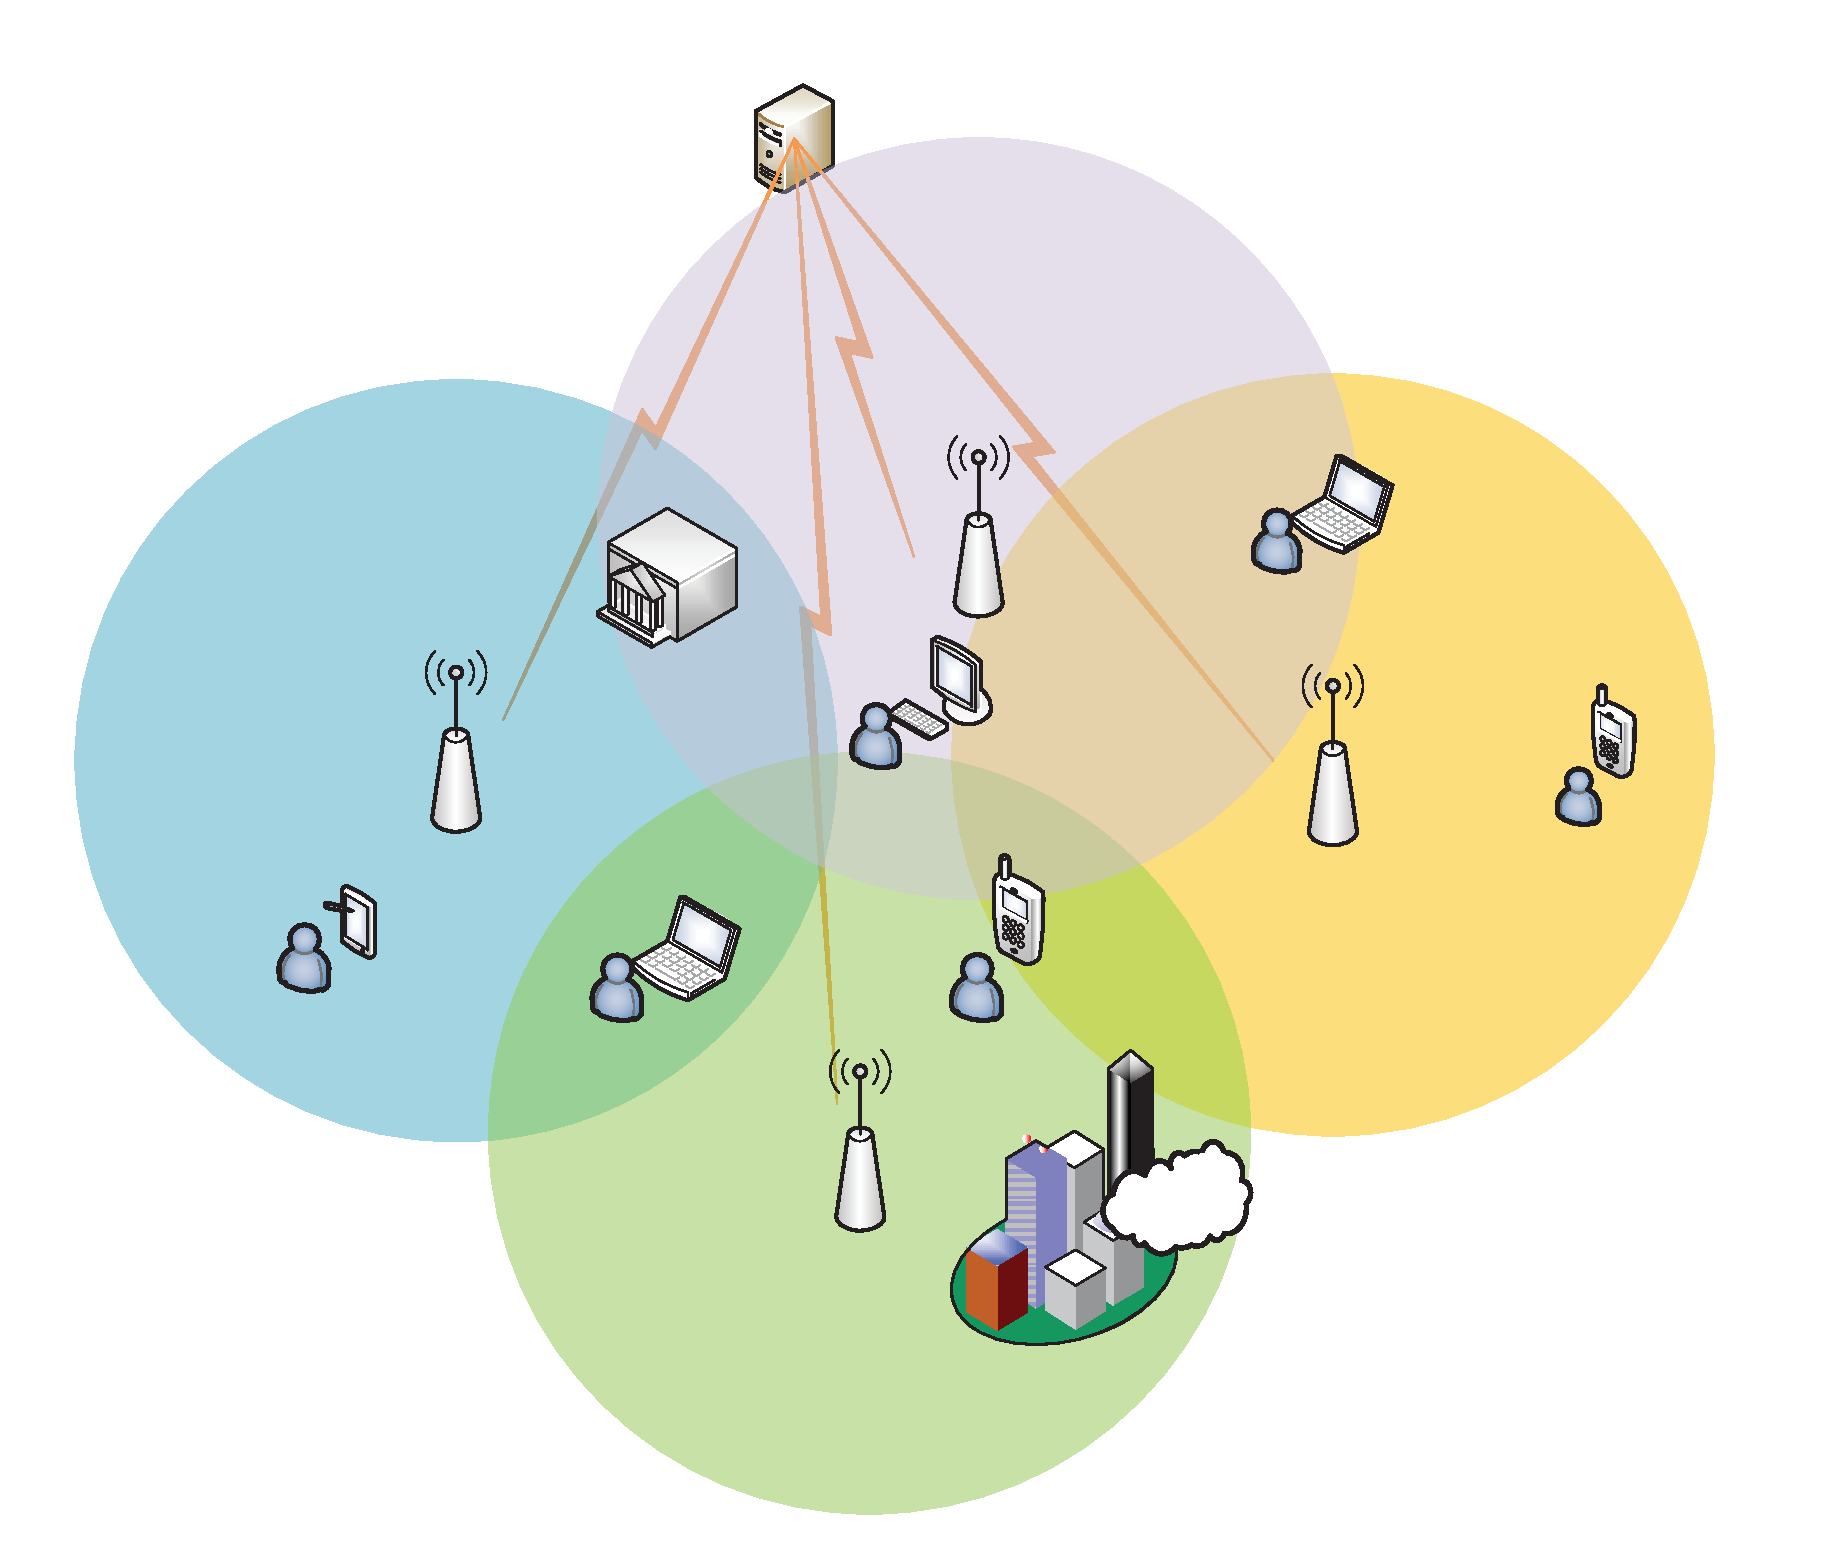
\includegraphics[width=8.5cm]{Fig1.eps}
\caption{A schematic map of Super Wi-Fi system.}
\end{figure}
\section{System Model}
In this section, before we illustrate the proposed POMDP algorithm,
we describe the system model of the Super Wi-Fi network.
As shown in Fig1., like in other wireless network,
the OU could observe multiple BSs, the number of which is denoted as \(N_A\).
In the network, users that only access one certain BS due to limitations like geographical distribution is called Passive User (PU).
For each BS, there is a maximum number of users that it could serve simultaneously due to limited spectrum,
as BS could not maintain the SINR for overcrowded users.
We use the notation \(N_U\) to represent the maximum number of users.
Thus, the user state in each BS could be denoted as \(S_U = i,\, i = \,0,\,1,\,...,\,N_U\).
Different from the discrete user state, the battery could be any continuous value between \(0\)
and the maximum battery value \(B_M\).
Note that in our work, The \(B_M\) and \(N_U\) for different BS could be different and our method still works.\\
\subsection{Access and Observation Model}
During each time slot, a certain quantity of energy, denoted as \(E_H\) is harvested,
and energy \(E_T\) is consumed during transmission.
Between adjacent time slots, new PUs may arrive and
old PUs may leave after finishing their service or the battery is not adequate for every service.
And thus a revised birth and death process is used to describe the process of user behaviors.
The transition probability of number of PUs is calculated as,
\begin{align}\label{formula1}
&\zeta\left(S_U'| S_U, Q_B, \Phi\right) = \nonumber\\
&\begin{cases}
	\lambda, &\mbox{if $Q_B$ is enough and $S_U' = S_U + 1$,}\\
	\mu S_U, &\mbox{if $Q_B$ is enough and $S_U' = S_U - 1$,}\\
	I_0\left(S_U'\right), &\mbox{if $Q_B$ is insufficient,}\\
	0, &\mbox{otherwise.}\\
\end{cases}
\end{align}
In the above equation, \(\lambda\) is the arriving rate and the \(\mu' = \mu S_U\) is the leaving rate of the process.
Note that when the battery is exhausted, all the users are dropped,
which is represented by the indication function \(I_0\left(S_U'\right)\),
i.e., \(S_U' = 0\) if battery is not enough.
Whether the \(Q_B\) is adequate or not is shown in the next subsection.
At the start of each time slot,
the OU could either decide to access or sense one of the BSs within its range.
When the OU decide to access the \(i^{th}\) BS, namely \(\Phi = \Phi_{a}^i\),
it sends a request signal to the chosen BS.
And if the BS has the requested battery for serving this extra requrest,
it will activate OU's transmission in this time slot.
% At the end of the transmission, the BS would attach the system state of him to the PU,
% so that the PU could keep the newest state of the BS for later use.
But there is also risk that the request fails because of low power and collision.
In this case, the BS will reject the request.
Whether the transmission is successful or not, the BS will feedback the user its system state with a short costless signal.
When collision happens, the energy is wasted due to low SINR.
% and send back a short message informing the BS of the BS's system state.
In order save time and energy, a more conservative idea is to sense the BS, i.e. \(\Phi_{s}^i\).
When the BS receives a sense signal,
it only transmits its system state to the user with neglectable energy consumption.
\subsection{Physical Battery Model}
The harvested energy \(E_T\) is determined by the environmental parameters,
which, in our case, is the sun light intensity.
Gaussian model has been proved effective in predicting sun light intensity \cite{gaussian,data}.
In a small time slot, denoted as \(T_L\), the average solar intensity remains unchanged.
In our work, the solar intensity \(W_e\) is assumed to be
Gaussian distributed with average intensity \(\mu_S\) and variation \(\sigma_S\), \(\mathcal{N}\left(x;\mu_S,\sigma_S\right)\).
The harvested energy is given as \(E_H = W_eJ_{op}V_{op}\Omega_ST_L\eta\),
where the \(J_{op}\) and \(V_{op}\) is the optimal operating point of the existing harvesting devices \cite{physic},
the \(\Omega_S\) is the number of solar cells and the \(\eta\) is the harvesting efficiency.
The transmitting energy is adjusted to make sure transmission with certain SINR.
It is important to note that, current feedback-based power adjustment algorithm
like Inner Loop Power Management is not valid as the system state changes during the time slots.
Here a static power management is implemented.
The power consumption in a BS is determined by number of PUs and the OU's action,
which is \(E_T = \Upsilon_T(S_U, Q_B, \Phi)\).
In most cases, the access of OU could be regarded as an extra PU for the BS, i.e., for BS \(i\),
\(\Upsilon_T(S_U, Q_B, \Phi = \Phi_{a}^{i}) = \Upsilon_T(S_U + 1, Q_B, \Phi \ne \Phi_{a}^i)\).
When the required battery is more than the BS's remaining battery,
the users with the higher priority is served.
In our case, the OU has the lowest priority.
Now we could define the event that \(Q_B\) is adequate as \(Q_B- \Upsilon_T(S_U, Q_B, \Phi) \leq 0\).
Thus the battery in the next time slot could be expressed as follow,
\begin{equation}
	Q_B' = \mbox{min}\{Q_B + E_H - E_T, B_M.\}
\end{equation}
To protect PUs from OU that uses up all the energy, the OU will not be served by BS in shortage of energy,
for example, BS with energy for only serving one user in one time slot.
\section{POMDP AP selection}
In Section \Rmnum{2} we describe the system model, it is clear that decision has to be carefully chosen.
There are several factors to be considered: the tradeoff between immediate reward and the long term reward and
the uncertainty of system state during decision making.
POMDP, which is recently developing as a strong tool to deal with decision making under uncertainty,
come as a perfect solution to this system.
However, before we could formulate our proposed algorithm, it is important to define our system state.
\subsection{Battery Transition}
In the implementation of EH powered BSs, the battery is a continuous value.
And in a POMDP, the states have to discrete.
Intuitively, we could use more battery states to represent the same battery volume,
but this brings much increase in the complexity of POMDP.
In our work, we convert the continuous battery quantity into \(N_B\) discrete battery states
\(S_B = \lfloor Q_B N_B / B_M \rfloor\). \(S_B\) could take values from level \(0,\,1,\,...,\,N_B - 1\).
In order to calculate the transition probability between adjacent battery states,
we assume the fluctuate of discrete battery state is quasi-static.
Under the assumption, for a given discrete battery state \(S_B\),
the residue energy \(Q_B - B_MS_B/N_B\) is uniformly distributed between \(\lbrack0,\,B_M/N_B\rbrack\).
Clearly errors are brought by this assumption,
but the quasi-static assumption is proven to be effective
and works well after many time slots \cite{data}.
We denote the battery state changing between time slot as \(\Delta_B = S_{B,'} - S_B\).
We define a event \(\xi_j\) to denote that the real battery quantity change is more than \(j\) but less than \(j+1\) levels.
\(\xi_j := \{j\leq N_B\frac{E_H - E_T}{B_M} \le j+1\}\)
Then the probability could be computed as follow,
\begin{align}&\mbox{Pr}\left(\Delta_B = i |\Phi, E_H, \xi_j \right)\nonumber\\
=&\begin{cases} N_B\frac{\left(E_H - E_T\right)}{B_M} -j, &\mbox{$i = j + 1$}\\
\left(j+1\right) -N_B\frac{\left(E_H - E_T\right)} {B_M}, &\mbox{$i = j$}\\
0, &\mbox{otherwise.}\\
\end{cases}
\end{align}
In the equation, as mentioned in previous section, \(E_T = \Upsilon_T(S_U, Q_B, \Phi)\).
The situation where the \(E_H - E_T \le 0\) is simply doing the mirror computation of the above equation.
When we consider the Gaussian distributed light density, the actual battery transition is then,
\begin{equation}\label{battery}
\begin{aligned}
	&\mbox{Pr}\left(\Delta_B = i |\Phi\right) = \\
	&\int_{\frac{iB_M}{N_B} + E_T}^{\frac{\left(i+1\right)B_M}{N_B} + E_T}
	\mbox{Pr}\left(\Delta_B = i |\Phi, E_H, \xi_i\right) \mathcal{N}\left(E_H;\bar{\mu_S},\bar{\sigma_S}\right) dE_H+\\
	& \int_{\frac{\left(i-1\right)B_M}{N_B} + E_T}^{\frac{iB_M}{N_B} + E_T}
	\mbox{Pr}\left(\Delta_B = i |\Phi, E_H, \xi_{i-1}\right) \mathcal{N}\left(E_H;\bar{\mu_S},\bar{\sigma_S}\right) dE_H.\\
\end{aligned}
\end{equation}
In the equation, the mean and variance of the Gaussian distribution are scaled accordingly after mutiplication.
\subsection{System Transition Probability}
When the user transition probability and battery transition probability is computable,
we could focus on the formulation of POMDP.
Note that the POMDP state is the system state, which contains state information of all BS.
To make the following math more readable and flexible,
two equivalent notation of system state is used simultaneously, i.e.
the centralized form of system state \(S\) and
the decentralized form of system state \(S_D = \{S_B^1,\,S_U^1,\,...,\,S_B^{N_A},\,S_U^{N_A}\}\).
\(S = 1,\,2,\, ... \,N_S\), where \(N_S = \left(N_BN_U\right)^{N_A}\) is the number of system state.
For the transition probability for a single BS,
the probability of \(S_U'\) and \(S_B'\) in the next slot are conditionally independent
given the current \(S_U\), \(S_B\) and \(\Phi\).
\begin{equation}
\begin{aligned}
	\mbox{P}\left(S_U',S_B'|S_U,S_B,\Phi\right) =
	\zeta\left(S_U'|S_U, S_B, \Phi\right) \delta\left(S_B'|S_U, S_B, \Phi\right)\\
\end{aligned}
\end{equation}
The \(\zeta\left(S_U'|S_U, S_B, \Phi\right)\) is given in equation \eqref{formula1}.
And the battery transition is calculated based on the equation \eqref{battery},
\begin{align}
	&\delta\left(S_B'|S_U, S_B, \Phi\right)\nonumber\\
	= &
	\begin{cases}
		\mbox{Pr}\left(\Delta_B = S_B' - S_B|\Phi \right) &\mbox{if $S_B' \le N_B - 1$,}\\
		\sum_{\Delta_B = S_B' - S_B}^{\Delta_B = \Delta_B^{Max}}\mbox{Pr}\left(\Delta_B|\Phi\right),
		&\mbox{if $S_B' = N_B - 1$.}\\
\end{cases}
\end{align}
In the case of battery overflow, \(S_B'=N_B - 1\), all the extra battery is abondoned.
We truncate the probability above \(\Delta_B^{Max}\) as they are as small as zero by \(4\) decimals.
The overall transition is computed as,
\begin{align}\label{transition}
	T\left(S'|S,\Phi\right) = \prod_{i = 1}^{i = N_A}\mbox{P}\left(S_B^{i,'}, S_U^{i,'}|S_U^i, S_B^i, \Phi\right)
\end{align}
\subsection{POMDP Optimal Algorithm}
In POMDP formulation, the OU only has the partial knowledge of the system.
At the end of each slot, the OU could get the BS's system state \(S_B^O\) and \(S_U^O\),
which we use \(\mathcal{O}\) to denote.
The observation probability function is given as follow.
\begin{align}
	Z\left(O|S',\Phi\right) = \mbox{Pr}\left(O|S_U^{t,'}, S_B^{t,'}\right) =
	I_{S_U^{t,'},S_B^{t,'}}\left(S_B^O, S_U^O\right)
\end{align}
\(S_B^{t,'}\) and \(S_U^{t,'}\) are the system state of the target BS next time slot.
The indicator function is either \(1\) or \(0\).
The reward is define as \(R = 1\) if the access succeeds, else \(R= 0\).
Then the value function of a single state is,
\begin{equation}
\begin{aligned}
	V_t^\Phi\left(S\right) = R\left(S,\Phi\right) +\gamma\sum\limits_{S'}T\left(S'|S,\Phi\right)V_{t-1}^\pi\left(S'\right),
\end{aligned}%\sum\limits_{O'}Z\left(O|S',\Phi\right)
\end{equation}
where \(\pi\) denotes the optimal action in that state.
As no full knowledge is held for the OU, we use a belief vector to denote the system belief
\(\beta = \lbrack \beta\left(S = 1\right),\,\beta\left(S = 2\right),\,...,\,\beta\left(S = N_S\right)\rbrack\).	
Then the particular policy tree with a certain belief \(\beta\) is given as
\begin{equation}
\begin{aligned}
	V_t^\Phi\left(\beta\right) = & \sum\limits_{S}R\left(S,\Phi\right)\beta\left(S\right) +\\
	&	\gamma\sum\limits_{S}\sum\limits_{S'}\beta\left(S\right)T\left(S'|S,\Phi\right)V_{t-1}^\pi\left(S\right).
\end{aligned}
\end{equation}
For simplicity, if we already know all the value function of at the time \(t-1\) during iterations,
a value vector \(\alpha_t^\Phi = \lbrack \alpha_t^\Phi\left(S = 1\right),\,
\alpha_t^\Phi\left(S = 2\right),\,...,\,\alpha_t^\Phi\left(S = N_S\right)\rbrack\)
could be used to simplify the value function as,
\(V_t^\Phi\left(\beta\right) = \sum\beta\left(S\right)\alpha_t^\Phi\left(S\right)\).
Note that for the same \(\Phi\) and \(t\), there are multiple possible \(\alpha\) vectors.
and the optimal action is
\begin{equation}
\begin{aligned}
	\pi\left(\beta\right) =
	\arg\underset{\alpha_t^\Phi}{\max}\sum\limits_{S}\beta\left(S\right)\alpha_t^\Phi.\\
\end{aligned}
\end{equation}
The corresponding value function could be calculated under action \(\pi\left(\beta\right)\).
However, the corresponding optimal policy is not as easy as it seems to be, as the \(\beta\) has a continous value.
But fortunately, note that the \(V_t\) could be regarded as the function value of \(\beta\) in a hyper coordinate,
the axis of which is the components of \(\beta\).
As each set of \(\alpha_t\) vector could be regarded as a set of parameters of a hyper linear function,
% the function value \(V_t\) is piecewise linear with the \(\beta_t\),
there is a dominated hyperplane structure in the model.
The continuous belief space is divided into several \(\alpha\)-vector-dominated hyperplanes.
The partition of belief space in time \(t\) could be calculated given all the dominating \(\alpha_{t-1}\).
The details of algorithm for solving the partition could be find in a well written tutorial \cite{pomdptool}.
At the end of the time slot, the OU will update its belief vector according to its observation.
\begin{align}
	\beta'\left(S'|\Phi, O\right) = \frac{\sum_{O}Z\left(O|S',\Phi\right)\sum_{S}
	T\left(S'|S,\Phi\right)\beta\left(S\right)}
	{\sum_{S'}\sum_{O}Z\left(O|S',\Phi\right)\sum_{S}T\left(S'|S,\Phi\right)\beta\left(S\right)}
\end{align}
\subsection{Suboptimal Access Policy}
The optimal POMDP solution could be calculated off-line within seconds when the number of states is small.
However, the use of POMDP method is limited when \(N_A\) is massive,
and when the environment parameters, like solar coefficients \(\mu_S\), \(\sigma\),
the birth rate \(\lambda\) and death rate \(\mu\) of PUs, changes quickly.\\
The POMDP formulation tries to maximize success access ration \(\eta_A = N_S/N_T\),
where \(N_S\) is number of success access and \(N_T\) is the number of all the time slots.
We propose a dual perspective of solving the problem, by focusing on the harvested energy.
We name it Energy Based (EB) Method.
The problem is reformulated as,
\begin{equation}
\begin{aligned}
	\underset{\Phi_t,t=0,\,...,\,N_T}{\max}\sum\nolimits_{t=1}^{N_T}\mbox{E}\lbrack\mbox{H}\left(\beta^T, \Phi_t\right)\rbrack,\\
\end{aligned}
\end{equation}
where the \(\mbox{H}\left(S^T, \Phi_T\right) = \sum\mbox{min}\left(E_H,\,E_T+B_M-Q_B\right)\)
is the overall harvesting energy of all the BSs combined.
Now a suboptimal could be proposed by maximizing the system's next-time-slot harvested energy.
\begin{equation}
\begin{aligned}
	\Phi_t\left(\beta\right) = \arg{\max}\,\,\mbox{E}\lbrack\mbox{H}(\beta^{t+1}, \Phi_t)\rbrack,\\
\end{aligned}
\end{equation}
When sense is the best action, the OU will choose to sense the BS that is not sensed for the longest time.
Due to the limited space, some key rationality of the EB method is summarized.
First of all, when the solar intensity is strong,
we could assume few PUs will be forced to leave the BS earlier because of OU.
And in most cases, the transmitting power \(E_T = \Upsilon_T(S_U, Q_B, \Phi)\).
Thus the reward will increase linearly with the harvested energy.
Second, the EB method is a unselfish method, which would sacrifice some reward,
but will protect the PUs and overall utility.
Third, the EB method could implement learning algorithm and adjust to quick changes of the environmental parameters,
which will be show in the journal version of this work.
\begin{figure}
\centering
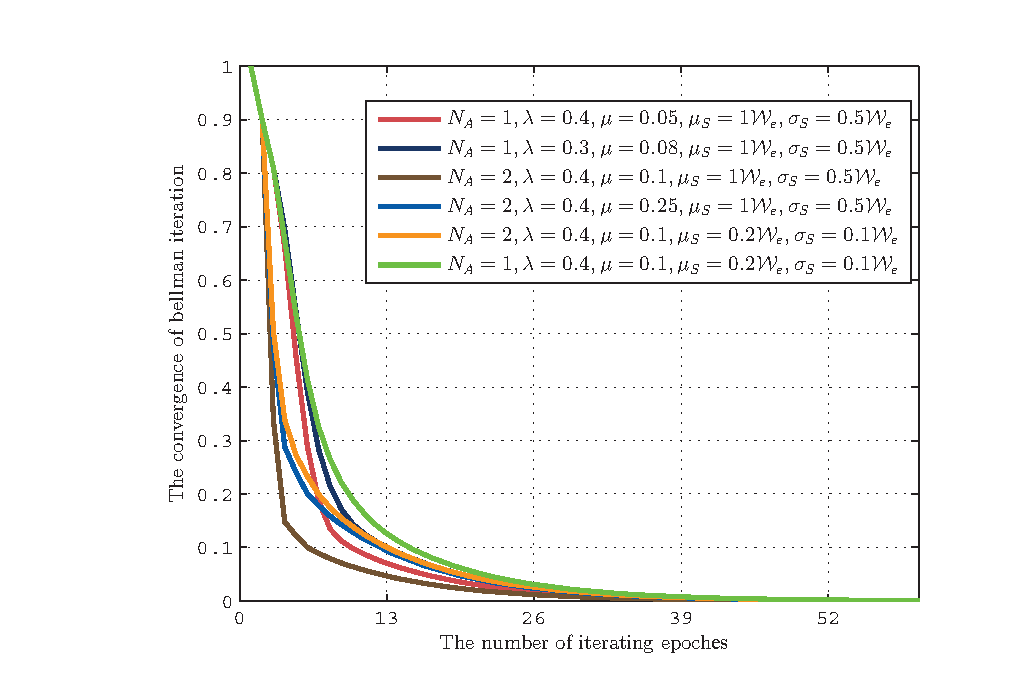
\includegraphics[width=8.5cm]{2_fig3.eps}
\caption{Illustration of the convergence of the POMDP iteration algorithm}
\end{figure}
\section{Simulation Results}
In this section, the convergence and effectiveness of the algorithm is illustrated.
In Fig.2, the convergence of the POMDP iteration algorithm is shown, where discount factor \(\gamma = 0.9\).
A bellman stoping criteria is used to determine the iteration stop.
In the figure the \(\alpha\) vector error shows the convergence of the iteration algorithm.
The POMDP simulation tool is provided by \cite{pomdptool}.
As is clear in the fig, the algorithm converges exponentially.\\
% ------------------------------------------%
\indent The effectiveness of the algorithm is calculated by comparing the \(\eta_A\)
during the overall time slots \(N_T = 10000\).
In the simulation, we use the parameters as follow.
The reference benchmark solar intensity is given as \(\mathcal{W}_e = 1\mbox{kW}/m^2\),
which is the average intensity on the surface of Earth\cite{electric}.
We use the work from \cite{circuit}, where the optimal power per benchmark solar intensity \(\mathcal{W}_e\)
is \(P_H = J_{op}V_{op} = 1.32\mbox{mW}/\mathcal{W}_e\), with a efficiency \(\eta = 75 \%\).
And there are \(\Omega_S = 40\) cells in one harvesting device.
The time slot length is \(T_L = 200\mbox{ms}\).
And as there is no corresponding industry implementation,
we assume a transmission power strategy \(E_T = \Upsilon_T(S_U, Q_B, \Phi)\)
that is proportional to the number of serving users,
which is rational considering a wide range wireless network with negligible between-user interference.
Transmission power for each user is \(P_T = 40\mbox{mW}\).\\
\indent In order to show the efficiency, several algorithms are implemented as comparisons.
CSMA/CA and CSMA/CD methods are used.
Slightly different to the standard CSMA, the OU senses the BSs instead of carrier.
And the algorithm tries to avoid collision and energy exhaust.
The CD method will stop request when failure detected. A exponential back-off algorithm is used.
After \(c\) failure, a random number of sleeping time slot between \(0\) and \(2^c - 1\) is chosen.
The CA method will only access after the user sense the BS and know that a successful service is available.
In random access algorithm, the OU simply chooses action with equal possibility.\\
\begin{figure}[t]
\centering
\subfigure[The utility ratio with arrival rate in single BS]{
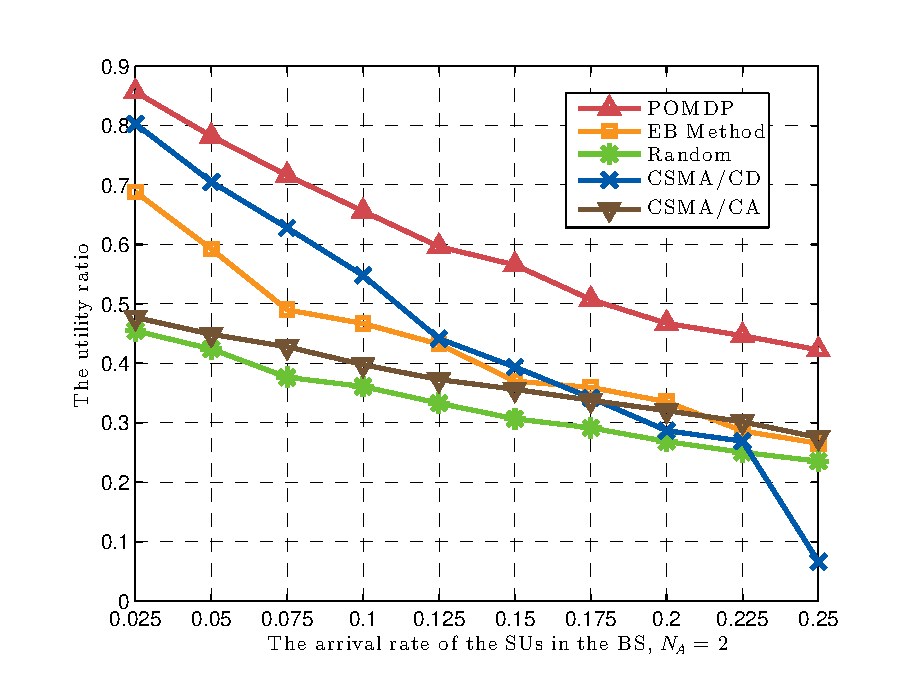
\includegraphics[width=0.5\textwidth]{3_fig1_1.eps}}
\subfigure[The utility ratio with solar intensity in single BS]{
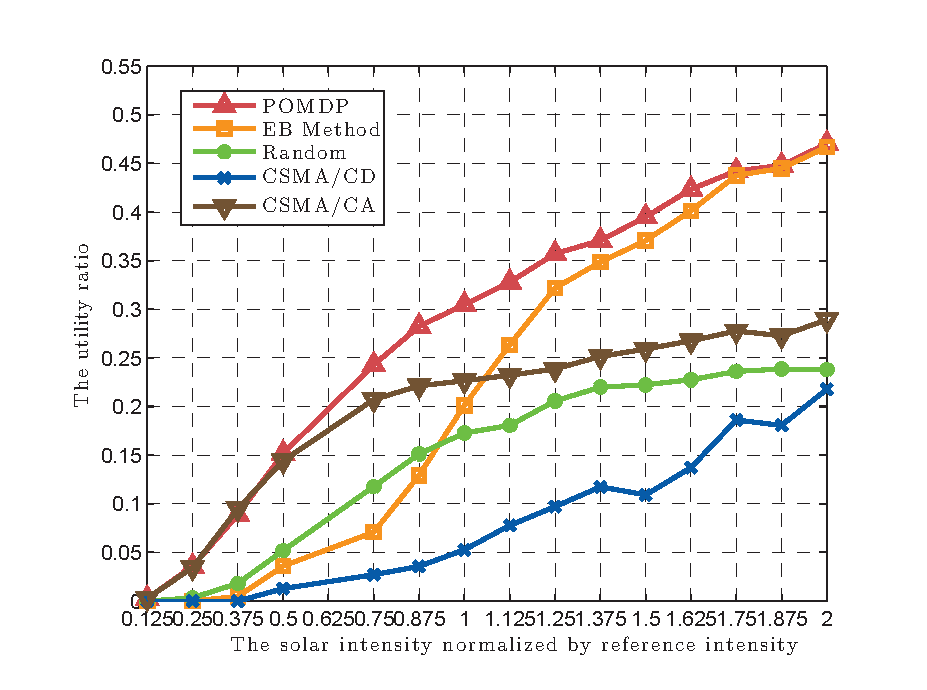
\includegraphics[width=0.5\textwidth]{3_fig2_2.eps}}
\caption{Single BS with \(S_U = 0,\,1,\,2,\,3,\, N_B = 8\)}
\end{figure}
\begin{figure}[t]
\centering
\subfigure[The utility ratio with arrival rate in two BS]{
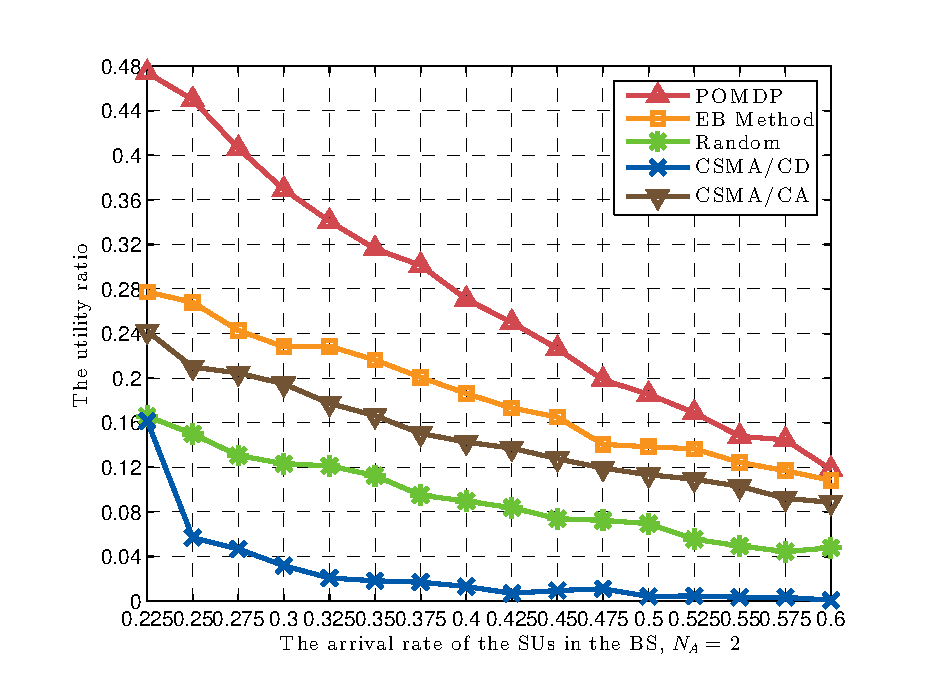
\includegraphics[width=0.5\textwidth]{3_fig2_1.eps}}
\subfigure[The utility ratio with solar intensity in two BS]{
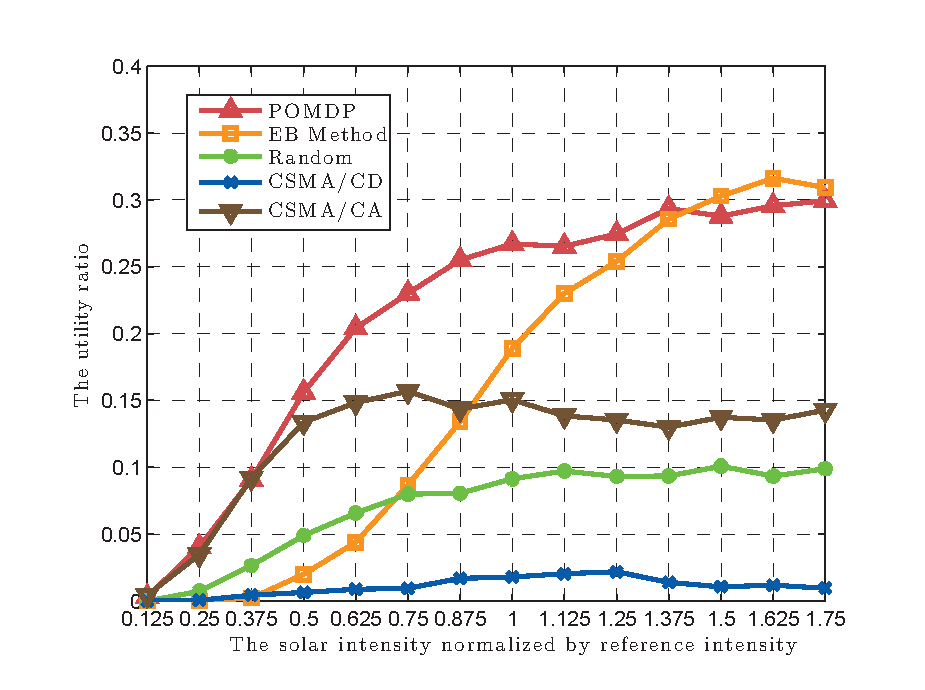
\includegraphics[width=0.5\textwidth]{3_fig1_2.eps}}
\caption{Two BS with \(U_N = 0,\,1,\, N_B = 3\)}
\end{figure}
\indent In Fig. 3, we consider single BS with possible number of user from \(0,\, 1,\, 2,\, 3\), \(N_B = 8\), \(B_M = N_BP_TT_L\),
and the leaving rate \(\mu = 0.05\). 
In Fig. 3 (a), the \(\mu_S = 1\) and \(\sigma_S = 0.5\), and in Fig. 3 (b), the arrival rate \(\lambda = 0.4\). 
As shown in the figure, the performance of proposed POMDP is significantly higher,
with the EM method's overall performance following at the second place,
which validates the efficiency of our algorithms.
From (a), the CSMA/CD method could have a good performance when the system is not busy,
but decreases quickly with the increasing arrival rate of PUs.
From (b), it is also clear that even when the solar intensity is strong, 
the traditional algorithms' ability to increase utility is still obviously limited.
As they are not able to make use of the EH information of the system.
It is also worth noting that, as we predicted, when the solar intensity is strong,
the suboptimal EB method will approach the proposed POMDP method.\\
\indent In Fig. 4, multiple BSs are considered, with possible number of user from \(0,\, 1,\), \(N_B = 3\), \(B_M = N_BP_TT_L\),
and the leaving rate \(\mu = 0.05\). 
Besides what we find in Fig. 3, we also find in Fig. 4 
that when the possible serving positions is limited, the crowded system make the CSMA/CD method almost useless.
In (b), when the solar intensity is small, the utility of CSMA/CD increases with intensity due to more available sources.
But when the solar intensity is big, 
the more solar intensity, the more OUs are staying in the BS, 
and thus the CSMA/CD has less chances of being served.
Also, in (b), the suboptimal EB method could overperform POMDP method when the intensity is big, 
which is mainly brought by the errors caused in the POMDP formulation, like using the quasi-static assumption.
\section{Conclusion}
In this paper, we proposed a powerful POMDP algorithm to solve the access problem in EH powered network,
which is promising and instructive in building a national range Super Wi-Fi network.
The framework given in this paper is adjustable to EH problems other than the Solar EH one.
A suboptimal EB method is proposed as well.
The affect of solar intensity, PU arriving rate, leaving rate and many other features are considered, 
proving our work reliable and effective.
And the future work of this paper focuses on the adjustment and prediction of system parameters.
\bibliographystyle{IEEEtran}
\bibliography{Ref}
\end{document}














In recent years, Super WiFi using IEEE 802.11af standard, was announced by the Federal Communications Commission (FCC), aiming to expand the coverage of wireless network access. Since the access points (AP) of Super WiFi will be deployed everywhere, the associated infrastructure including backhaul and energy supply system have to be simplified as much as possible to decrease the deployment cost. Wireless backhual has been proved to be able to substitute traditional wired backhaul \cite{30}. While for the power supply problem, constant battery replacement comes with high labor cost and additional administrative fee. The recent energy harvesting (EH) technology provide with an ideal solution for the power supply problem in Super WiFi. Wireless network service supplied by EH is equipped with devices that could harvest ambient energy including piezoelectric, thermal, solar energy etc. Some preliminary studies have been done on the applications of EH wireless network service, addressing the modification that is required to the current WLAN standard for better support \cite{27}. \\
%%%%%%
\indent In Super WiFi networks, when confronted with many APs, how a user makes the AP selection is a critical issue. Especially, when it comes to AP supplied by solar energy, the energy condition of each AP should be taken into account, besides quality of service (QoS). In order to solve the selection problem, many researches have been done in the literature. Markov Decision Process (MDP) has been used in AP selection game, e.g., some strategies, challenges and solutions were summarized in \cite{23}. As AP selection is a typical game problem \cite{22}, game theory has also been used as an effective approach. In \cite{7}, the selection problem was formulated from a pricing game perspective. Meanwhile, the characteristic of negative externality was considered in \cite{5} and \cite{21}, where a maximum number of access users for each AP was set and the utility is closely related with the number of access users. When it comes to AP selection algorithm, a no regret algorithm was designed in \cite{11} to help users to select among distributed APs. For the EH wireless network service, it has been widely studied as in \cite{17,18,19}. In \cite{17}, the authors characterized the indoor light energy availability and studied the energy allocation. In \cite{18}, the routing algorithms were explored from a network topology aspect. An opportunistic routing protocol was studied in \cite{19}, and the authors compared the proposed protocols with non-opportunistic protocols in wireless sensor networks using ambient energy harvesters (WSN-HEAP).\\
\indent However, all the existing works on network service selection have not considered the situation of APs supplied by ambient power. Apparently, for Super WiFi, EH is the most feasible way that could solve the energy supply problem. In addition, the previous works have separated the APs and users, i.e., either focusing on the transmitting strategies of the APs, or the users' access strategies, by assuming the other part is stable or invariant. However, in practical EH based networks, users are changing in number and distribution, as well as the APs' energy status and channel conditions. Therefore, APs and users are affecting each other, and should be considered simultaneously. Considering these problems, we focus on the problem of AP selection game in a wireless network service powered by ambient solar energy, which has a promising industry future as a key component in Super WiFi. Specifically, we formulate the user model and AP's battery model, considering their interaction effect and the battery physical features through MDP formulation. The optimal AP selection strategy is obtained by a designed value iteration algorithm.\\
\indent The rest of this paper is organized as follow. We describe the system model In Section \Rmnum{2}. The optimal selection based on MDP model is presented in Section \Rmnum{3}, including the battery model, user access model and the AP selection algorithm. In Section \Rmnum{4}, we evaluate the performance of our proposed approach. Finally, Section \Rmnum{5} draws the conclusion.

\section{System Model}
In this section, we describe the overall picture of the EH based Super WiFi system and how we model the problem. As shown in Fig. 1, a Super WiFi system consists of \(N\) APs that are supplied by solar energy harvesting is considered. The APs of the system are connected to the server through wireless backhaul. In each time slot, new arriving users can access one of the available APs and stay connected until he/she leaves the associated AP. In the system, we assume that each AP has a maximum number of accessed users \(U_M\), i.e., if a user intends to access a AP whose accessed user number \(U_i = U_{M}\), the access will be denied. For the AP's battery condition, it is quantized into several discrete levels, where the maximum number of levels is denoted as \(B_M\).\\
\indent Since the number of the users accessing one AP and the battery quantity of that AP are different from those of other APs, the QoS one AP provides is also quite different from others'. If we denote the quantized battery level of the \(i^{th}\) AP as \(B_i\), then the utility of the users defined as the individual throughput, can be written by
\begin{equation}
R_i = W_i \log\left(1 + \frac {P_T(U_i, B_i) / N_0} {(U_i-1)P_I/N_0+1}\right) ,
\end{equation}
where \(B_{i} \in \{ j \mid j = 0,1,...,B_M - 1\}\) and \(U_{i} \in \{ i \mid i = 0,1,...,U_M\}\). In the expression, the $W_i$ is the bandwidth, \(N_0\) is the noise power, which we assume to be the same between every AP and users and remain constant all the time. The signal-to-noise power ratio is \({P_T(U_i, B_i)}/ {N_0}\) and the interference-to-noise power ratio is \({P_I} / {N_0}\). The \(P_T(U_i, B_i)\) is the function of the power used to transmit the pockets to users of the AP. The transmitting power of the APs usually increases with the battery level and the user number. The exact expression is beyond the discussion of this work, which is stipulated by the using WLAN standards \cite{29} and studied in \cite{25}.\\
% % %

\section{AP Selection Strategy based on MDP}
\indent In this section, we analyze users' AP selection strategy in EH based Super WiFi networks. Usually, after a user access one specific AP, he/she would stay connected for a period of time, and thus the long-term utility that can be obtained within this period should be considered. Therefore, we use MDP model to formulate this AP selection problem. Here, the system state is defined as both the user number staying in one AP and the remaining battery quantity. In the following, we will first discuss how we formulate the user states and the battery states, and then propose a value iteration algorithm to derive the optimal strategy.
\subsection{Battery Model}
\indent Quantization of the battery quantity to an appropriate number of levels is necessary. There is a trade off between the accuracy of the algorithm and the amount of the states. In our evaluation, four or five levels of battery conditions would return a result that is accurate enough and not having a big algorithm complexity.\\
\begin{figure}[t]
\centering
\includegraphics[width=8.5cm]{figure1.eps}\\
\caption{A schematic map of Super WiFi system, and a common system model of a solar cell.}
\end{figure}
\indent If the duration \(T\) of the time slot is small enough, a battery level could only switch from a level to its adjacent levels at the end of each time slot in a discrete time system. The transition of a level to its neighbour is simultaneously determined by the energy the AP harvests and the energy it consumes when transmitting pockets. As, given the system state, the transmitting power is already known, the following part of this subsection demonstrates the formulation of relationship from the battery level to the harvesting power.\\
\indent The harvesting power is determined by the illumination and the battery level. In this paper, a classic physical model of the photoelectric battery was used, showed in Fig. 1. The harvesting power first increases with the voltage and then decreases to zero when the maximum voltage is reached, as is showed in Fig. 2. Considering the ideal model of the solar cell, the relation between the current and the voltage are given in \cite{2} as
\begin{equation}
\begin{aligned}
J(V) = J_{SC} - J_o\left(e^{\frac{qV} {k_B T_\kappa}} - 1\right),
\end{aligned}
\end{equation}
where the \(k\) and \(T_\kappa\) is the boltzmann's constant and temperature. In the equation, \(J(V)\) is the current density. When illuminated area and the number of cells connected in one harvesting device is constant, the scale factor \(\rho\) from \(J\) to harvesting power is only linearly affected by illumination level \(\zeta\). In a specific period of the day, \(\zeta\) could be regarded as Gaussian distributed with an average illumination intensity. When time slot \(T\) is small enough, the illumination could be regarded as invariable in each time slot. And if we denote the distribution center of \(\rho\) with the average illumination level \(\bar{\zeta}\) as \(\bar{\rho}_\zeta\), the probability density function of \(\rho\) is given as
\begin{equation}
\begin{aligned}
f_{\rho}(x) = \frac {1} {\sqrt {2\pi}\sigma} e ^{-\frac {(x-\bar{\rho}_\zeta)^2} {2 {\sigma}^2}},
\end{aligned}
\end{equation}
where \(\sigma\) is the standard deviation.
The battery quantity of the \(i^{th}\) battery level \(B_i\) is approximated as \(\overline {B_i}\) and from the electrical formula between voltage and energy quantity in a capacitor, we have \(V = \sqrt{ \frac{2 \overline{B_i}} {C}}\). Thus the function of harvesting power with the voltage is is given as
\begin{equation}
\begin{aligned}
P_H(B_i) = \rho\left(J_{SC} - J_o\left(e^{\frac{qV / C} {k_B T}} - 1\right)\right) \cdot V,
\end{aligned}
\end{equation}
Thus the relation between the battery level and the harvesting power is formulated. \\
\indent For denotation convenience, the \(k^{th}\) APs in the Super Wifi system is refer to as AP \(k\), where \(k \in \{ 1,2,3,...,N \}\). As the transmitting power and harvesting power are known, spontaneously, we could give the transition probability of the battery level of AP \(k\) from level \(i\) to level \(j\) after each time slot, where \(0 \le j \le B_{M} - 1\), and \(0 \le i \le B_{M} - 1\).
\begin{align}
&\beta_{k}(j\mid i,U_k) =\\
&\quad\begin{cases}
\mbox{Pr}\{P_H(k) - P_T (U_k, i) >  {\Delta B_{i,j}}  /T  \}, &\mbox{if $j=i+1$},\\
\mbox{Pr}\{P_T (U_k, i) - P_H(k) > {\Delta B_{j,i}}  /T  \}, &\mbox{if $j=i-1$ },\\
0, &\mbox{if $|j-i|>1$},\\
1 - \sum_{m=0, m\ne i}^{m = B_{M} -1}\beta_{k}(m\mid i), &\mbox{if $j=i$},
\end{cases}\nonumber
\end{align}
where the \(\Delta B_{i,j}\) is the average battery quantity difference between the battery level \(i\) and \(j\).
\begin{figure}
\centering
\includegraphics[width=8.5cm]{figure2.eps}\\
\caption{The current density versus voltage curves and the harvesting power of a cell versus the voltage. The key parameters, \(J_{SC} = 13.364\mbox{mA cm}^{-2}\) and \(V_{OC} = 0.7631\mbox{V}\) is obtained from the work done by Hsiang-Yu Chen \cite{3}.}
\end{figure}
\subsection{User Model}
In the Super WiFi system, two kinds of users are considered. One is self-directed users (SDU) such as the mobile phone users that have several APs in its reach. They could decide which AP to access, and they arrive at a rate of \(\lambda_0\). And the other kind is passive users (PU), for example, the fixed temperature sensors in hospitals. They could only access one specific AP unless the AP is full. For the AP \(k\), its PUs arrive with Poisson arrival distributed rate \(\lambda_{k}\). And the departure rate of all the users in APs is exponential distributed with parameter \(\mu\). To make the formulation clear and concise, we construct a fiducial transition probability from user state \(i\) to user state \(j\) not considering other SDUs and conflicts as follow,
\begin{equation} \psi_{k}(j \mid i) =
\begin{cases}
\lambda_k(1 - i\mu), &\mbox{if $j=i+1,$}\\
i\mu(1 - \lambda_k), &\mbox{if $j=i-1,$}\\
0, &\mbox{if $|j-i|>1.$}\\
\end{cases}
\end{equation}
The total system state including all the APs inside is denoted as a vector \(S = (B_1,U_1,B_2,U_2,...B_N,U_N)\). Given the system states, the SDUs will choose their optimal strategy denoted as \(\pi(S)\). When the conflict of PUs happens, a re-access is carried out. When a PD failed to access an AP because it is full, he/she will be immediately send to a available new AP chosen by the Super Wifi system. A greedy re-access protocol is used by the system. The stand-by AP is given by
\begin{equation}
\begin{aligned}
\xi(S)=\arg\underset{i < B_{M}}{\max}\, W_i \log\left(1 + \frac {P_T(U_i + 1, B_i) / N_0} {(U_i)P_I/N_0+1}\right).
\end{aligned}
\end{equation}
The probability of conflict of a full AP \(k\) in the next time slot is \((1-U_M \mu)\lambda_k\). Thus, the fiducial transition probability could renew into the real transition probability as below:
\begin{equation}
\begin{aligned}
\psi_{\xi(S)}(i+1 \mid i)= &\psi_{\xi(S)}(i+1 \mid i) +\\
&\sum_{m = 1,U_m = U_M}^{N}(1-U_M \mu) \lambda_m,\\
\end{aligned}
\end{equation}
\begin{equation}
\begin{aligned}
\psi_{\pi(S)}(i+1 \mid i) = \psi_{\pi(S)}(i+1 \mid i) + \lambda_0,
\end{aligned}
\end{equation}
and the probability that the system would remain the same is calculated as,
\begin{equation}
\begin{aligned}
\psi_{\pi(S)}(i \mid i) = 1 - \sum\nolimits_{m=0, m\ne i}^{m = B_{M} -1}\psi_{k}(m\mid i).\\ %\qquad\mbox{if $j=i$}.\\
\end{aligned}
\end{equation}
The final system transition probability is defined as follow:
\begin{equation}
\begin{aligned}
P(S'\mid S) = \prod\limits_{k=1}^N \psi_{k}(U_k' \mid S)\beta_{k}(B_k' \mid S).
\end{aligned}
\end{equation}
\subsection{Expected Utility}
A MDP over infinite horizon is considered to obtain the utility of the users. As the PUs are heteronomous, we consider the selection of AP for SDUs. A SDU can not change his AP after accessing, and we use \(\gamma\) to denote the accessed AP. The utility until he leaves is denoted as \(V_{\gamma}(S_0)\). Then his expected utility could be given as,
\begin{equation}
\begin{aligned}
V_{\gamma}(S_0) = E \left(\sum\limits_{t=0}^\infty (1-\tau)^t R_{\gamma}(S_t)\Bigg| S_0\right).
\end{aligned}
\end{equation}
Here \(1 - \tau\) is the discount factor. For iteration algorithm, the equation above could also be written in a recursive way \cite{26},
\begin{equation}
\begin{aligned}
V_{\gamma}(S_0) = R_{\gamma}(S_0) + (1-\tau) \sum\limits_{S'}P_{\gamma}(S'|S_0)V_{\gamma}(S').
\end{aligned}
\end{equation}
Given that the SDU accesses and stays in \(\gamma\), the fiducial transition probability \(\psi_{k}(j \mid i)\) is not the same as the equation (5), but
\begin{equation}
\psi_{k}(j \mid i, \gamma) =
\begin{cases}
\lambda_k(1- (i - 1)\mu), &\mbox{if $j=i+1,k = \gamma$},\\
\lambda_k(1- i\mu), &\mbox{if $j=i+1,k \neq \gamma$},\\
(1 - \lambda_k)(i - 1)\mu, &\mbox{if $j=i-1, k = \gamma $},\\
(1 - \lambda_k)i\mu, &\mbox{if $j=i-1, k \neq \gamma$},\\
0, &\mbox{if $|j-i|>1$}.
\end{cases}
\end{equation}
To solve the real transition probability, the strategy of newcome SDUs is needed. In system \(s\), the strategy of newcome SDUs is given as,
\begin{equation}
\begin{aligned}
\pi_s = \arg \underset {k \leq N}{\max} \ V_{k}(s'),
\end{aligned}
\end{equation}
where \(s'\) is the system state that is different to \(s\) only in that \(U_k' = U_k + 1\), as the access of the AP \(k\) will lead the system state from \(s\) to \(s'\). With the optimal strategy obtained, the transition probability could be calculated by applying equations (8) to (10). In order to solve the MDP iteration, we use the algorithm showed in the table above, which is a revised form of value iteration, first used in \cite{5}.\\
\indent As no SDUs could gain a higher expected utility by not choosing the optimal strategy in the profile, the optimal strategy meets a Nash equilibrium.
\begin{algorithm}[t]
\caption{Value iteration algorithm}
\label{alg}
\begin{algorithmic}
\STATE /********Initialization*********/
\STATE Initialize the \(V_k^{(0)}(s)\leftarrow 0\) for all \(s \in \mathcal{S}\), \(k \in \mathcal{AP}\)
\STATE Initialize the \(\pi^{(0)}(s)\leftarrow 1\) for all \(s \in \mathcal{S}\), \(k \in \mathcal{AP}\)
\STATE /***********Iteration**********/
\WHILE{\(\max\limits_s \mid V_k^{(t)}(s) - V_k^{(t+1)}(s)\mid >\epsilon\)}
\STATE for all \(s \in \mathcal{S}\), \(k \in \mathcal{AP}\)
\STATE {\( V_k^{t+1}(s) \leftarrow R_{k}(s)\ \)+ \\
\(\qquad\qquad\qquad(1-\tau)\sum\limits_{s'}P_{k}(s'|s,\pi^t)V_k^t(s')\).}
\STATE \(\pi^{(t+1)}(s) \leftarrow \arg\underset{\gamma \leq N}{\max}\, V_{\gamma}(\tilde{s})\),\\
            where \(s'\) is the system state different \\
            \qquad\qquad\qquad from \(s\) only in that \(U_k' = U_k + 1\)
\ENDWHILE
\STATE /***********Output***********/
\STATE \( \pi^{\ast}(s) \leftarrow \pi^{t+1}(s)\).
\STATE \( V^{\ast}(s) \leftarrow \underset{\gamma \leq N}{\max}\, V_{\gamma}(\tilde{s})\).
\end{algorithmic}
\end{algorithm}
\section{Simulation Results}
\begin{figure}
\centering
\includegraphics[width=8.5cm]{newResult2.eps}\\
\caption{The convergence of the MDP value iteration.}
\end{figure}
In this section, the convergence and effectiveness of the proposed algorithm are illustrated. In the effectiveness simulation, myopic strategy and random strategy are used as comparations. The myopic strategy is the strategy that SDU users will access the AP that could provide the maximum immediate reward, namely, \(\pi_s^{myopic} = \arg \underset {k \leq N}{\max} \ R_{k}(s)\). The random strategy is that the SDUs will access random AP that is in the Super WiFi system, i.e. \(\mbox{Pr}\{\pi_s^{rand} = i\} = \frac {1} {N}\). According to model and analysis in the Section \Rmnum{2}, \Rmnum{3}, we ascertain several important coefficients. Firstly, same battery quantity differences between the adjacent battery levels is used, i.e. dividing the battery quantity into isometric discrete battery levels. The parameters of the solar cell in \cite{3} is used. As the maximum voltage and storage vary with the number of cells, in this simulation, four power coefficients are of the same order. The charging power \(\max \, P_{H}\), the energy gap between adjacent battery levels divided by the time \(\Delta B / (T \cdot N_0)\), and the power \(P_T\), \(P_I\) are of the same order. We have \(P_T / N_0 = 10\), \(P_I / N_0 = 10\), \(\Delta B / (T \times N_0) = 6\) and \(\max P_{H} / N_0 = 6,...,10\) when \(\bar{\zeta} = 6 \zeta_{Unit},...,10\zeta_{Unit}\). The simulation was operated 10000 times to avoid random error. \\
\indent In Fig. 3, the convergence of the MDP value iteration was illustrated. The Fig. 3(a) is a picture illustrating the sum of \(\mid V_k^{t+1}(s) - V_k^{t}(s)\mid^2\), for all \(s \in \mathcal{S}\), \(k \in \mathcal{AP}\). And Fig. 5(b) illustrates the number of different AP selections between adjacent iterations. From the \(15^{th}\) iteration, the selection strategy remains the same after every iteration and the result is not drawn in the Fig. 3(b). The figure shows that our MDP converges in an exponential way.\\
\indent In Fig. 4, the performance versus arrival rate of the SDUs \(\lambda_0\) and the leaving rate \(\mu\) is evaluated. The coefficients are \(\lambda_1 = \lambda_2 = \lambda_3 = 0.1\),\ \(N = 3\) APs, with \(U_i = 0, 1,...,4\) and \(B_M=4\), \(\zeta = 10 \zeta_{Unit}\). In Fig. 4(a) \(\mu = 0.1\), and in Fig. 4(b) \(\lambda_0 = 0.1\). It is showed in the figure that the proposed strategy has an evident advantage over the myopic one, and random strategy performs the worst. In Fig. 4(a), the myopic utility is set to 1 and normalized the other two accordingly. In Fig. 4(b), the utility decreases with departure rate, as users stay shorter in the system. When \(\mu\) gets bigger, the proposed strategy has less advantage over the myopic. Because a shorter stay time results in more importance of immediate reward.\\
\indent Fig. 5 shows the performance of different strategies under different illumination level. The parameters are \(\lambda_0 = \lambda_1 = \lambda_2 = \lambda_3 = 0.1\), \(\mu = 0.1\), \(N = 3\) APs, and \(U_i = 0, 1,...,4\), \(B_M=4\). All the strategy has a trend of expecting a higher utility as there is more solar energy. And the proposed strategy has a stable advantage over the other two.\\
\begin{figure}
\centering
\includegraphics[width=8.5cm]{newResult1.eps}\\
\caption{The performance of the proposed strategy, myopic strategy and the random strategy is evaluated versus the arrival rate of the SDUs and the departure rate of the users in the APs.}
\end{figure}
\section{Conclusion}
In this paper, we have studied the selection problem of AP in Super WiFi powered by solar energy with negative externality. We in this work formulate the user number and the battery level of each AP as Markov states. We successfully construct the transition probability and use value iteration algorithm to solve the optimal selection strategy in MDP. The result of our proposed algorithm shows that our formulation and algorithm are correct and reliable, with the proposed strategy having a stable and evident outperformance. Our work could be instructive for the development of Super WiFi, providing an effective selection strategy.
\begin{figure}
\centering
\includegraphics[width=8.5cm]{newResult3.eps}\\
\caption{The different performance of three strategies under different illumination levels.}
\end{figure}

